\chapter{Corte CNC}

\textbf{*}Este capítulo estará enfocado en fresado CNC, pues es la tecnología disponible en el Campus. El contenido es complementario a la experiencia técnica a adquirir en los laboratorios.

\section{Introducción}

La fabricación sustractiva por corte se basa en la remoción controlada de material para dar forma a un volumen, utilizando una o varias \textbf{herramientas de corte}.

Este tipo de tecnología es la automatización de máquinas tradicionales de manufactura metalmecánica, principalmente tornos y fresadoras. Un torno produce piezas con simetría cilíndrica mediante la rotación del material base, mientras que una fresadora ofrece una mayor versatilidad en cuanto a las geometrías que puede alcanzar, al usar una herramienta rotativa móvil en varios ejes. Así, las máquinas CNC más comunes son los tornos y fresadoras CNC, o bien los centros de mecanizado, que combinan ambas capacidades en una sola unidad. 

\begin{figure}[h!]
	\centering
	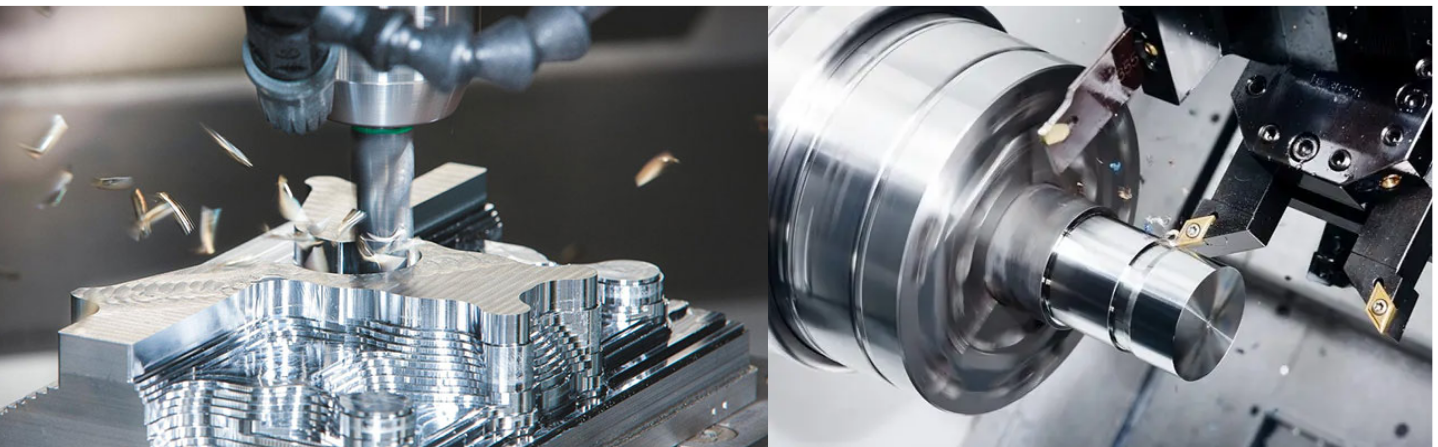
\includegraphics[width=1.0\linewidth]{imgs/tornoyfresa.png}
	\caption{Fresado a la izquierda, torneado a la derecha. \href{https://www.weerg.com/}{Fuente}}
	\label{tornoyfresafig}
\end{figure}

A diferencia de las tecnologías aditivas, frecuentemente asociadas al prototipado, el corte CNC ofrece una vía directa hacia la \textbf{producción de piezas finales}, pues permite trabajar con una gama más amplia de \textbf{materiales técnicos de ingeniería}, lograr mejores \textbf{acabados superficiales} y alcanzar \textbf{tolerancias más estrictas}. Esto permite \textbf{fabricar prototipos funcionales y soluciones reales}, con propiedades mecánicas adecuadas para su implementación en servicios exigentes.

Otra diferencia fundamental con respecto a la impresión 3D radica en que el proceso no altera de forma significativa las propiedades mecánicas del material base, ya que no implica fusión, solidificación ni cambios térmicos intensos como en muchas tecnologías aditivas. Por tanto, el análisis de estos procesos se centra principalmente en aspectos como la \textbf{calidad dimensional}, la \textbf{productividad} del mecanizado y el \textbf{desgaste de las herramientas}, factores clave para la optimización de costos y la eficiencia del proceso.

En comparación con los procesos de fabricación en serie, como el moldeo por inyección o el troquelado, el corte CNC ofrece una menor eficiencia en términos de producción a gran escala. Sin embargo, presenta ventajas clave en cuanto a flexibilidad, reducción de tiempos de preparación y menor inversión inicial.

Por otro lado, los procesos de fabricación en serie suelen requerir la elaboración de moldes maestros de alta precisión para la conformación de piezas y productos. Estos elementos, fundamentales rara vez se fabrican mediante otro método que no sea el mecanizado CNC de alta calidad, debido a los exigentes requerimientos de tolerancia, acabado superficial y estabilidad dimensional que demandan para lograr vidas útiles extensas.

Como veremos en los siguientes capítulos, estas características dependerán principalmente de los \textbf{parámetros de corte}, de los \textbf{atributos de la máquina}, de la \textbf{herramienta de corte}, de las \textbf{propiedades del material}, y de las \textbf{estrategias del proceso}. 

\section{Fabricación por corte de viruta}

La acción de una herramienta de corte sobre un material puede derivar en 3 mecanismos, dependiendo de las propiedades del material, la herramienta y los \textbf{parámetros de corte}, los cuales son:

\begin{enumerate}
	\item \textbf{Deformación plástica}: El material es forzado a fluir localmente más allá de su límite elástico, lo que permite la generación de viruta. Este es el mecanismo típico en metales dúctiles.
	
	\item \textbf{Fractura frágil}: El material se rompe debido a la propagación de grietas, generalmente sin deformación previa significativa. Común en materiales cerámicos, vidrios, o compuestos duros.
	
	\item \textbf{Abrasión}: Remoción superficial del material por desgaste mecánico, sin necesidad de fractura macroscópica o fluencia plástica. Característico de procesos como rectificado o pulido.
\end{enumerate}

Por lo general, los modelos de corte para fresado o torneado se referirán al primer mecanismo, pues es más fácil de modelar, y se le denominará \textbf{arranque de viruta}. La abrasión se estará relacionada con procesos de rectificado o pulido, los cuales también pueden ser implementados en CNC.

Para que ocurra efectivamente el corte, es decir, la generación de viruta y la penetración de la herramienta en el material, deben cumplirse ciertas condiciones fundamentales, principalmente una \textbf{condición geométrica} (que deriva en una condición \textbf{cinemática}) y otra de \textbf{resistencia del material}.

La condición geométrica para que se inicie el arranque de viruta, exige que el espesor de corte supere un umbral mínimo que permita activar el mecanismo plástico de corte. En primera aproximación, esta condición se expresa como:

\begin{equation}
	h > 0
\end{equation}

donde $h$ es el \textbf{espesor no deformado de la viruta}, que depende del avance y la geometría de la herramienta. Sin embargo, en la práctica (especialmente en procesos de microfabricación) existe un espesor mínimo efectivo, $h_{\text{min}}$, por debajo del cual el material no se corta adecuadamente (Figura \ref{filofig}). En lugar de producirse una viruta, el filo genera:

\begin{itemize}
	\item \textbf{Rubbing} (frotamiento): contacto superficial sin corte, con generación de calor por fricción.
	\item \textbf{Ploughing} (arado): desplazamiento plástico del material hacia los lados, sin separación efectiva.
\end{itemize}

\begin{figure}[h!]
	\centering
	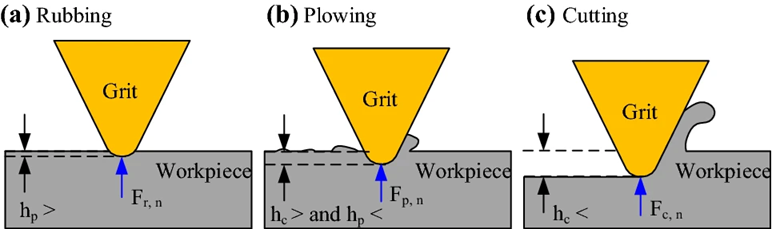
\includegraphics[width=0.9\linewidth]{imgs/filo.png}
	\caption{Comportamiento del material frente a la profundidad de corte: a) Frotamiento b) arado y c) corte. \href{https://link.springer.com/article/10.1007/s40684-020-00199-2/figures/5}{Fuente}}
	\label{filofig}
\end{figure}


Estas condiciones aumentan el desgaste de la herramienta, deterioran la calidad superficial y reducen la eficiencia del proceso de mecanizado. De esta forma, la condición se transforma en:

\begin{equation}
	h > h_{min}
\end{equation}

Esta penetración está determinada por la \textbf{cinemática del corte}, es decir, por la relación entre la velocidad de avance de la herramienta y su velocidad de rotación. Esta relación se expresa a través del parámetro conocido como \textbf{avance por diente}, definido como:

\begin{equation}
	f_z = \frac{v_c}{z \cdot N}
\end{equation}

donde:
\begin{itemize}
	\item $f_z$ es el \textbf{avance por diente} [mm/diente],
	\item $v_c$ es la \textbf{velocidad de avance} de la herramienta [mm/min],
	\item $z$ es el \textbf{número de dientes activos} de la herramienta,
	\item $N$ es la \textbf{velocidad de rotación} [rpm].
\end{itemize}

Este parámetro representa la distancia que avanza cada diente en una revolución, y por tanto determina el \textbf{espesor no deformado de viruta} $h$. Si $f_z$ es menor que el espesor mínimo de corte $h_{\text{min}}$, no se genera viruta adecuadamente, y el proceso entra en los regímenes no deseados de rubbing o ploughing.

En consecuencia, el avance por diente debe mantenerse por encima de ese umbral mínimo, el cual depende del material, la geometría del filo y las condiciones de corte. No obstante, $f_z$ también está limitado por la capacidad de la herramienta y por los requisitos de \textbf{calidad superficial} y \textbf{tolerancias}. Un avance excesivo puede generar virutas muy gruesas, sobrecargar el filo y deteriorar la precisión del mecanizado. Por tanto, se debe encontrar un equilibrio adecuado que permita un corte efectivo sin comprometer la calidad ni la integridad de la herramienta.

Por otro lado, la herramienta debe aplicar una fuerza tangencial suficiente para vencer la resistencia del material a ser cortado. Esta condición se expresa como:

\begin{equation}
	F_c \geq \tau_s \cdot A
\end{equation}

donde:

\begin{itemize}
	\item $F_c$ es la fuerza de corte aplicada.
	\item $\tau_s$ es el esfuerzo de corte específico del material.
	\item $A = h \cdot b$ es el área de corte, siendo $b$ el ancho de contacto de la herramienta con el material.
\end{itemize}

\begin{figure}[h!]
	\centering
	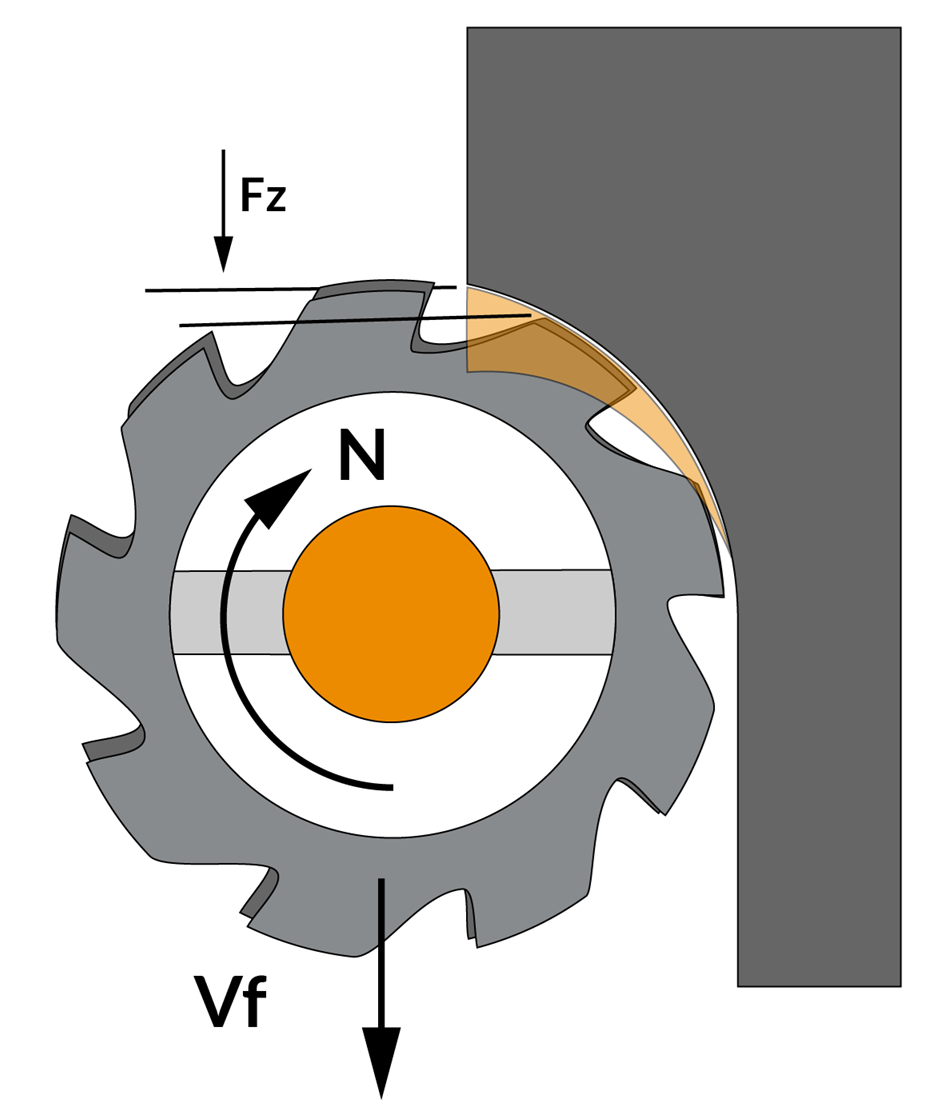
\includegraphics[width=0.4\linewidth]{imgs/fpt.png}
	\caption{Diagrama del avance de la herramienta. \href{https://fmcarbide.com/pages/milling-feed-rate}{Fuente}}
	\label{fptfig}
\end{figure}

Nótese que esta condición está relacionada con la dureza, pues estamos ante un fenómeno de indentación local. Así, mientras más duro es una material, menor es su \textbf{maquinabilidad}, una característica que indica la facilidad de mecanizado. Cómo veremos más adelante, este atributo dependerá además de otras propiedades del material base. 

Estas condiciones son las mínimas para que el fenómeno de remoción ocurra, no obstante, no puede ser llevado a cabo por cualquier maquinaria. De esta manera, el proceso va a ser viable además si es que la potencia de la maquinaria lo permite. La potencia de corte requerida se calcula como:

\begin{equation}
	P_{\text{corte}} = F_c \cdot v_c
\end{equation}

donde:

\begin{itemize}
	\item $v_c$ es la velocidad de corte (tangencial),
	\item $F_c$ es la fuerza de corte.
\end{itemize}

Así, la condición energética sobre el hardware se expresa como:

\begin{equation}
	P_{\text{disponible}} \geq P_{\text{corte}}
\end{equation}

Si expandimos los términos de 4.5 usando 4.4, se tiene:

\begin{equation}
P_{corte}=\tau_{s}\cdot A \cdot v_{c} = \tau_{s} MRR
\end{equation}

Donde $MRR$ es la tasa de remoción de material (\textit{material removal rate} $\mathrm{[mm^{3}]}$). De esta manera, la limitación en potencia implica un \textit{trade-off} entre la dureza del material a maquinar y la productividad del proceso.

Las condiciones nombradas previamente serán entonces las mínimas para seleccionar una máquina dado un proceso, no obstante, no son suficiente si queremos considerar además la calidad de fabricación. La calidad estará determinada por la respuesta dinámica del sistema (vibraciones) y la transferencia de calor.

La \textbf{estabilidad dinámica del sistema herramienta–pieza–máquina} es fundamental para asegurar una buena calidad de mecanizado y prolongar la vida útil de la herramienta. Durante la operación, el sistema puede excitarse por perturbaciones externas o internas (como la descomposición del corte en viruta), generando \textbf{vibraciones autoinducidas} conocidas como \textit{chatter} (Figura \ref{chaterfig}). Este fenómeno ocurre cuando pequeñas oscilaciones en la herramienta se amplifican debido a una realimentación positiva entre las fuerzas de corte y el desplazamiento relativo entre herramienta y pieza.

Estas vibraciones pueden causar:

\begin{itemize}
	\item Ruido excesivo y pérdida de precisión dimensional.
	\item Daños en el filo de la herramienta.
	\item Mal acabado superficial.
	\item Desgaste prematuro de componentes de la máquina.
\end{itemize}

\begin{figure}[h!]
	\centering
	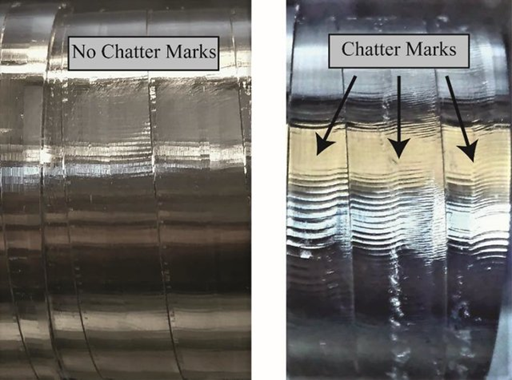
\includegraphics[width=0.7\linewidth]{imgs/chatter.png}
	\caption{Superficie maquinada estable e inestable (\textit{chattering}). \href{https://www.researchgate.net/publication/327415504_MECHANICS_DYNAMICS_AND_STABILITY_OF_TURN-MILLING_OPERATIONS}{Fuente}}
	\label{chaterfig}
\end{figure}

Parte del comportamiento dinámico del sistema está determinado por la \textbf{rigidez estructural} de la máquina (incluyendo el chasis, la transmisión y los soportes), así como por la capacidad de \textbf{control de torque} de los motores de la transmisión. En este sentido, incluso si la máquina dispone de la potencia requerida para realizar el corte, una rigidez insuficiente o un control deficiente pueden comprometer la \textbf{precisión dimensional} de la pieza mecanizada.

Otra consideración esencial es la \textbf{transferencia de calor generada por el corte}, ya que una parte importante de la energía consumida se convierte en calor en la zona de corte. Este calor se distribuye entre:

\begin{itemize}
	\item La herramienta (puede causar pérdida de dureza, desgaste o incluso falla).
	\item La pieza (afectando tolerancias o propiedades metalúrgicas).
	\item La viruta (que idealmente debería llevarse la mayor parte del calor).
\end{itemize}

El exceso de temperatura puede provocar:

\begin{itemize}
	\item Deformación térmica de la pieza y de la herramienta.
	\item Reducción de la vida útil de la herramienta.
	\item Cambios microestructurales (luego, en las propiedades) no deseados en la pieza y en la herramienta.
\end{itemize}

Por esta razón, las máquinas de corte CNC suelen incorporar un subsistema de \textbf{refrigeración activa}. 

En consecuencia, los procesos de corte CNC deben ser abordados como sistemas multivariables, en los que intervienen de manera interrelacionada las propiedades del material, las características geométricas y dinámicas de la máquina, las condiciones de corte y el tipo de herramienta utilizada. Para un material dado, la elección de los parámetros de operación no puede realizarse de forma aislada, sino que debe considerar la compatibilidad entre todos estos elementos.

Es importante destacar que una limitación geométrica inherente al mecanizado CNC con herramientas rotativas es la imposibilidad de generar esquinas internas perfectamente rectas. Debido a la forma cilíndrica de estas herramientas, todo borde interno presentará inevitablemente un radio mínimo, determinado por el radio del filo de corte.

\section{Subsistemas, herramientas y accesorios}

\subsection{Subsistemas}

Un subsistema esencial en todo sistema CNC es el de \textbf{fijación del material base} (\textit{stock}) que será maquinado. Este subsistema asegura la estabilidad y la precisión del proceso, evitando desplazamientos durante la operación.

 Los dispositivos de fijación pueden variar considerablemente según el tipo de material y la máquina utilizada. En máquinas simples, donde la mesa de trabajo es un consumible, el stock puede fijarse directamente a través tornillos o adhesivos. En cambio, en aplicaciones más exigentes, se emplean dispositivos como prensas de tornillo (Figura \ref{tormachfig}), mordazas mecánicas o sistemas de fijación neumáticos automatizados, los cuales pueden sincronizarse con el ciclo de operación para evitar interferencias o colisiones con la herramienta.
 
 Deben tomarse dos precauciones importantes de acuerdo al sistema de fijación:
 
 \begin{itemize}
 	\item Considerar los elementos de fijación en la configuración del CAM, para evitar colisiones.
 	\item La presión de fijación podría inducir deformaciones en el material.
 \end{itemize}
 
 \begin{figure}[h!]
 	\centering
 	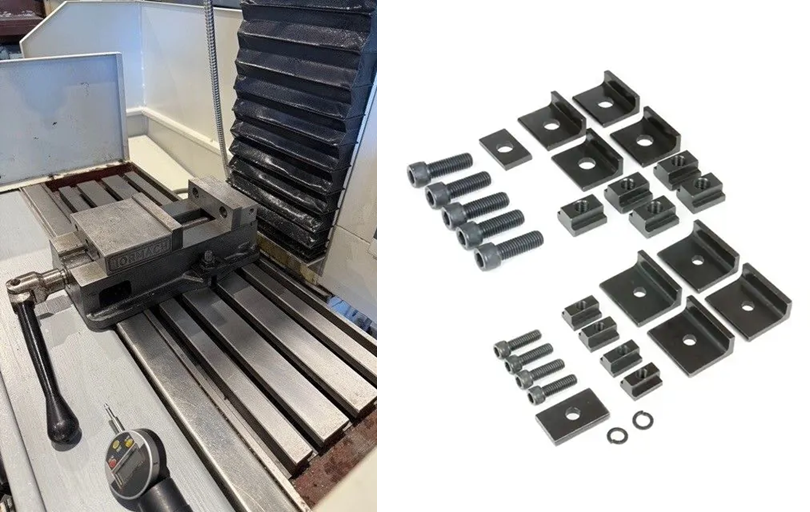
\includegraphics[width=0.8\linewidth]{imgs/tormach.png}
 	\caption{A la izquierda, prensa en mesa de trabajo de una CNC Tormach, a la derecha, accesorios de fijación. \href{https://tormach.com}{Fuente}}
 	\label{tormachfig}
 \end{figure}
 
Cuando las geometrías de las piezas son complejas o requieren alta precisión, se emplean \textbf{fixtures} personalizados para sujeción y posicionamiento. Estos dispositivos aseguran la estabilidad y repetibilidad durante el proceso, minimizando deformaciones y movimientos no deseados. Los fixtures se diseñan específicamente según la pieza o familia de piezas, garantizando una fijación adecuada que permite alcanzar las tolerancias requeridas en la fabricación.

 \begin{figure}[h!]
	\centering
	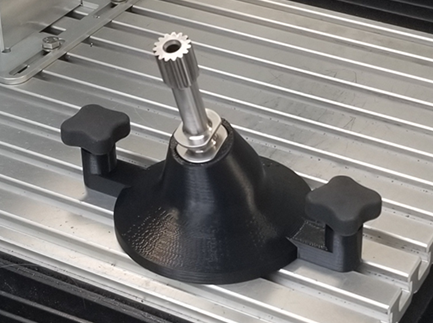
\includegraphics[width=0.5\linewidth]{imgs/jig.png}
	\caption{Soporte personalizado impreso en 3D. \href{https://stratasys.com}{Fuente}}
	\label{jigfig}
\end{figure}

 Un componente central del subsistema de corte en una máquina CNC es el \textbf{husillo} (\textit{spindle}), encargado de transmitir el movimiento rotacional a la herramienta (Figura \ref{husillofig}). Su función principal es generar y mantener la velocidad de corte requerida en el punto de contacto entre la herramienta y el material. A diferencia de otros actuadores rotacionales presentes en equipos automatizados, el husillo en procesos de mecanizado está sometido a elevadas exigencias dinámicas y estructurales, ya que debe operar a altas velocidades bajo carga, soportando simultáneamente esfuerzos radiales, axiales y térmicos.
 
 
  \begin{figure}[h!]
 	\centering
 	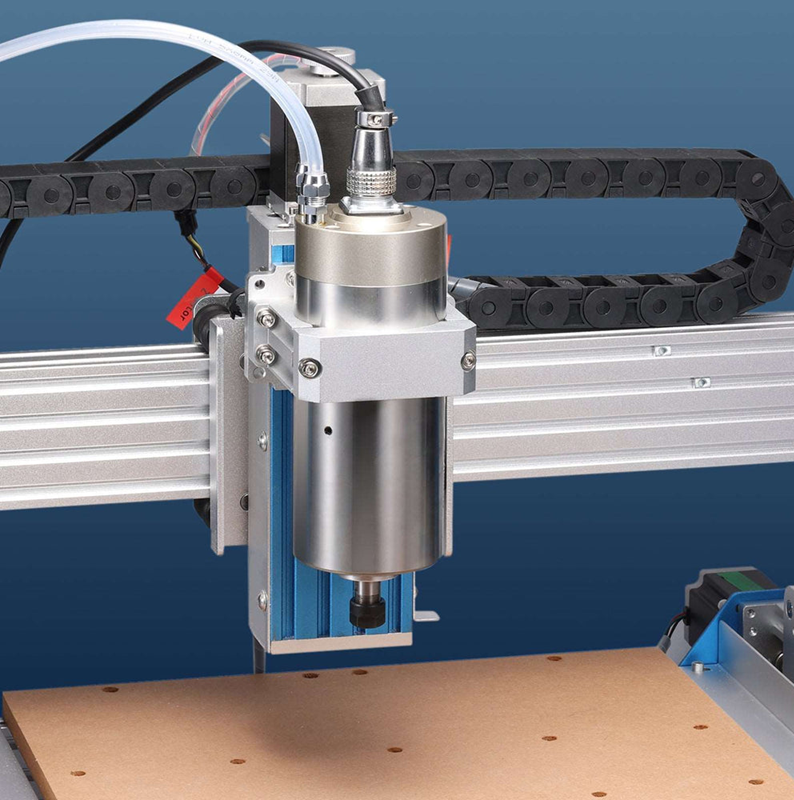
\includegraphics[width=0.5\linewidth]{imgs/husillo.png}
 	\caption{Husillo en máquina CNC de baja escala. \href{https://www.sainsmart.com/products/water-cooled-spindle-motor-kit}{Fuente}}
 	\label{husillofig}
 \end{figure}
 
 Los husillos pueden clasificarse según su fuente de accionamiento (eléctrico o neumático), el rango de velocidad, el sistema de transmisión (directa, por correa o por engranajes) y la capacidad de carga. Los husillos modernos incorporan sensores de temperatura, vibración y velocidad, lo que permite al sistema CNC adaptar dinámicamente las condiciones de corte.
 
El husillo determina la compatibilidad con los \textbf{portaherramientas}, lo que a su vez define la variedad y versatilidad de procesos que la máquina CNC puede ejecutar. 

Dado que los procesos CNC generalmente involucran múltiples herramientas con longitudes distintas, es necesario contar con un método para definir y compensar los \textit{offsets} de cada herramienta en relación con un sistema de coordenadas común. Una técnica frecuente consiste en establecer una referencia inicial mediante una herramienta montada en el husillo, la cual se aproxima hasta hacer contacto con una superficie definida de la pieza o de la máquina. Este contacto puede detectarse mediante el cierre de un circuito eléctrico, utilizando la conductividad del material como mecanismo de detección.

En el caso de materiales no conductores, se emplea una placa auxiliar de espesor conocido que actúa como interfaz de contacto; dicho espesor se considera luego en el cálculo del offset. En sistemas con cambio automático de herramienta, las herramientas se miden e identifican previamente y sus datos se cargan al sistema de control. De este modo, a partir de una única referencia inicial, la máquina puede operar de forma continua sin requerir pausas para recalibración entre herramientas.

Finalmente, si el sistema de medición automática no está disponible o presenta fallas, como último recurso el procedimiento se realiza manualmente: la herramienta se aproxima cuidadosamente hasta tocar una lámina de espesor conocido ubicada sobre el material base, y se ajusta el offset de forma manual considerando dicho espesor.

Los sistemas de refrigeración activa no solo cumplen la función de disipación térmica, sino que además aportan:

\begin{itemize}
	\item \textbf{Evacuación de la viruta}: facilita el despeje continuo de la zona de corte, evitando la acumulación de material y posibles interferencias.
	\item \textbf{Amortiguación de vibraciones}: contribuye a estabilizar el sistema al reducir pequeñas oscilaciones mecánicas.
	\item \textbf{Lubricación}: disminuye la fricción entre la herramienta, la viruta y la superficie mecanizada, reduciendo el desgaste.
	\item \textbf{Protección superficial}: forma una película que ayuda a prevenir la corrosión y el daño en componentes de la máquina y en la pieza de trabajo.
\end{itemize}

  \begin{figure}[h!]
	\centering
	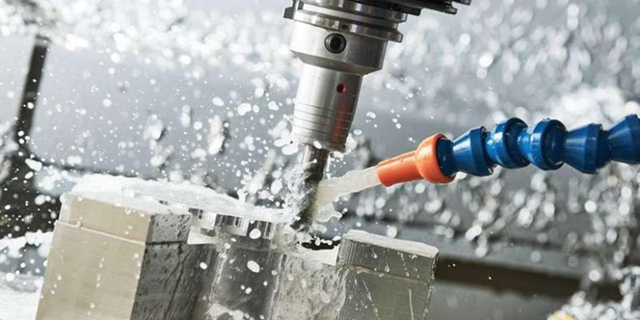
\includegraphics[width=0.7\linewidth]{imgs/cul.png}
	\caption{Refrigeración por chorro. \href{https://waykenrm.com/blogs/types-of-cnc-coolants/}{Fuente}}
	\label{culfig}
\end{figure}

El subsistema de \textbf{evacuación de viruta} en máquinas CNC puede adoptar diferentes configuraciones según el tipo de material y las características de la máquina. En equipos que procesan materiales con baja higroscopicidad, como metales, es común el uso de canales por los que circula el refrigerante, el cual arrastra las virutas hacia un sistema de filtrado. Allí, los residuos sólidos se separan y el refrigerante puede recircular en el sistema.

En cambio, cuando se trabaja con materiales que absorben humedad, como madera o polímeros espumosos, o bien en máquinas de menor tamaño, se prefiere la aspiración por vacío como método de recolección, ya que estos materiales pueden degradarse o hincharse en contacto con fluidos refrigerantes.

\subsection{Herramientas}

Las herramientas de corte utilizadas en máquinas CNC presentan una amplia variedad de tipos, geometrías y materiales, cada uno adecuado para distintas operaciones y condiciones de mecanizado. Según su función principal, pueden clasificarse en \textbf{fresas}, \textbf{brocas} y \textbf{herramientas especializadas}. Las \textbf{fresas} poseen filos de corte distribuidos principalmente en el manto o periferia, lo que las hace adecuadas para operaciones laterales y de desbaste en múltiples ejes. En cambio, las \textbf{brocas} están diseñadas para realizar cortes axiales (perforaciones verticales), concentrando el filo en la punta.

Dentro de las fresas, que constituyen las herramientas más utilizadas en centros de mecanizado, se pueden distinguir subtipos según su geometría de corte (Figure \ref{fresifig}). Las más comunes son:

\begin{itemize}
	\item \textbf{Fresas planas} (flat end mills): de uso general, ideales para desbaste y acabado de superficies planas o cavidades con bordes rectos.
	\item \textbf{Fresas esféricas} (ball end mills): utilizadas principalmente para el mecanizado de superficies 3D, curvas complejas o contornos suaves, donde se requiere alta resolución geométrica.
	\item \textbf{Fresas toroidales} (bull nose): con una punta redondeada que combina características de las planas y esféricas, útiles para transición suave entre superficies.
\end{itemize}

  \begin{figure}[h!]
	\centering
	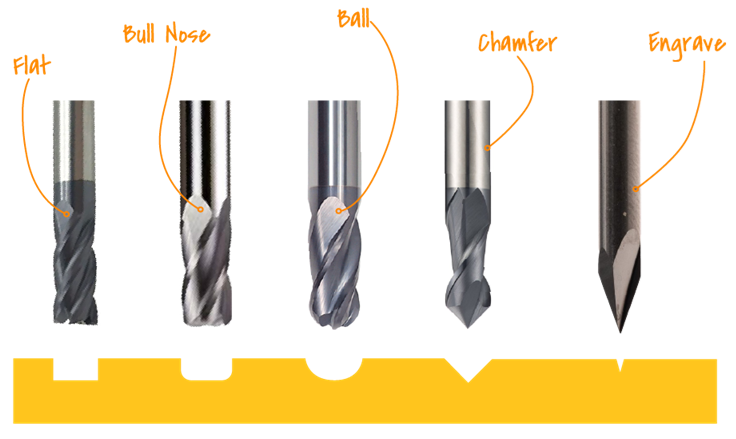
\includegraphics[width=0.8\linewidth]{imgs/fresi.png}
	\caption{Tipos comunes de fresas. \href{https://www.making.unsw.edu.au/learn/cnc-module2/}{Fuente}}
	\label{fresifig}
\end{figure}


Las características principales de una herramienta se ilustran en la Figura \ref{anatomifig}. Entre los parámetros más relevantes se encuentran:

\begin{itemize}
	\item \textbf{Diámetro}: determina tanto la resolución geométrica alcanzable como la tasa máxima de remoción de material. El diámetro de corte puede diferir del diámetro del vástago (shank), relevante para fijar la herramienta al portaherramienta.
	\item \textbf{Longitud total y longitud útil}: definen la profundidad máxima de corte y la rigidez efectiva de la herramienta durante la operación.
	\item \textbf{Filos}: El número de filos (flutes) y la dirección de la helice, influyen en la evacuación de viruta, la calidad de superficie y la eficiencia del corte.
\end{itemize}

El \textbf{ángulo de hélice} en una fresa determina la inclinación de los filos de corte respecto al eje longitudinal de la herramienta, afectando la dirección y eficiencia de la evacuación de viruta, así como las fuerzas generadas durante el mecanizado. 

Un \textbf{ángulo de hélice cero} (fresa recta) produce una carga de corte más brusca, con viruta fragmentada y pobre evacuación, siendo útil solo en aplicaciones específicas como plásticos duros o ciertos compuestos. Ángulos altos (40–45) generan una acción de corte más progresiva y suave, reducen la carga radial y mejoran el acabado superficial, pero disminuyen la rigidez del filo; se prefieren en materiales dúctiles como aluminio. En cambio, ángulos bajos (20–30) aumentan la rigidez de corte, siendo más adecuados para aceros duros y titanio. 

\begin{figure}[h!]
	\centering
	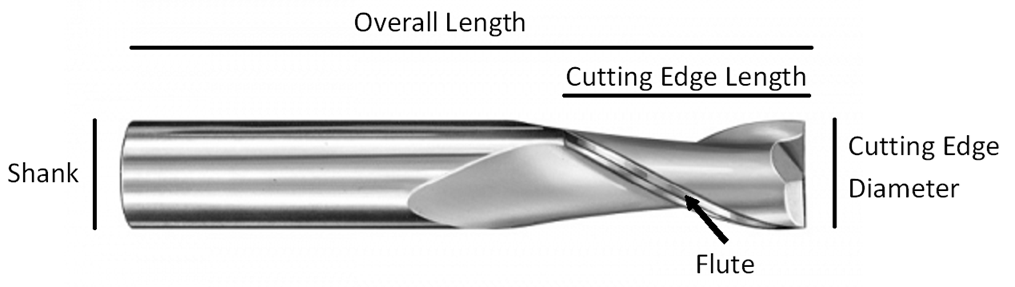
\includegraphics[width=0.8\linewidth]{imgs/anatomi.png}
	\caption{Partes de una fresa plana. \href{https://www.endmill.com.au/blog/choosing-the-right-end-mill-for-the-job/}{Fuente}}
	\label{anatomifig}
\end{figure}

Respecto a la dirección de hélice, las \textbf{hélices derechas} son las más comunes y expulsan la viruta hacia arriba (fuera del corte), mientras que las \textbf{hélices izquierdas} la empujan hacia abajo, siendo preferidas cuando se busca aumentar la estabilidad de la pieza, o evitar el levantamiento en piezas delgadas, o delaminación en materiales compuestos. 

Las herramientas pueden ser fabricadas en una sola pieza o mediante un cuerpo portador con \textbf{insertos de corte reemplazables}. Estos insertos, fabricados generalmente de carburo sinterizado o materiales cerámicos, permiten extender la vida útil del cuerpo de la herramienta y optimizar los costos operativos. En cuanto a materiales, las herramientas suelen estar hechas de acero rápido (HSS), carburo cementado (WC-Co), cerámicos o incluso diamante policristalino (PCD), según los requerimientos de velocidad, durabilidad y resistencia al desgaste.

La rigidez estructural y dureza de la herramienta no sólo es fundamental para mantener las condiciones ideales de corte, sino que determinan directamente la fuerza máxima de corte que puede ejercer, y luego, el MRR máximo. Una herramienta flexible o inadecuada puede inducir vibraciones, desviaciones geométricas y deterioro prematuro de la pieza y del filo (incluso fractura temprana), comprometiendo la precisión del mecanizado.

En procesos que exigen alta estabilidad térmica, pueden emplearse fresas con \textbf{refrigeración interna}, las cuales canalizan el fluido refrigerante directamente hacia la zona de corte, mejorando la evacuación de viruta y el control de temperatura.
 
\subsection{Accesorios}

El portaherramientas (tool holder) es el componente que fija la herramienta de corte al husillo de una máquina CNC, y su compatibilidad depende del tipo de vástago de la herramienta. Existen diversos sistemas de sujeción; por ejemplo, el sistema ER utiliza un collet elástico que puede adaptarse a un rango específico de diámetros de vástago (Figura \ref{er25fig}). Otros portaherramientas, como los diseñados para brocas con vástago cilíndrico o cónico, se ajustan a dimensiones fijas. En el caso de herramientas con cambio rápido, se emplean portabrocas específicos como el portabrocas de cierre rápido (keyless chuck).

  \begin{figure}[h!]
	\centering
	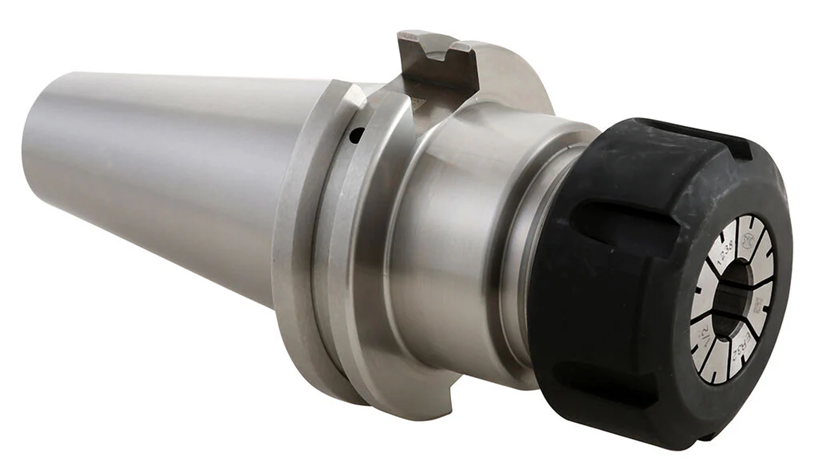
\includegraphics[width=0.5\linewidth]{imgs/er25.png}
	\caption{Portaherramientas ER25, se observa el mandril o portabroca, la tuerca y el collet. \href{https://shop.techniksusa.com/cnc-machining-center-tooling-accessories/collet-chucks/cat40-er-collet-chuck/22245}{Fuente}}
	\label{er25fig}
\end{figure}


En máquinas CNC básicas, el portaherramientas se acopla directamente al husillo, lo que limita la versatilidad del sistema a un único tipo de sujeción. En cambio, las máquinas de mayor gama utilizan un sistema de portacono (taper adapter), que actúa como interfaz entre el husillo y diversos portaherramientas intercambiables. Este sistema permite cambiar herramientas de forma más eficiente, sin necesidad de desmontar el portaherramientas completo.

Cuando se utilizan múltiples herramientas durante un proceso, es necesario definir un offset (desfase) para cada herramienta, ya que sus longitudes y geometrías pueden variar. Realizar este ajuste manualmente en cada arranque puede resultar ineficiente y propenso a errores. Por ello, muchas máquinas CNC modernas incorporan sistemas automáticos de medición de herramienta, capaces de identificar la longitud y el diámetro de la herramienta montada, integrando estos datos en la memoria del sistema. Si el programa CAM está correctamente configurado con las identificaciones de cada herramienta, la asignación de offsets se realiza automáticamente al iniciar la operación.

Además, el uso de instrucciones G-code y desplazamientos manuales permite redefinir las referencias de trabajo para distintas operaciones. Sin embargo, cuando se requiere mayor precisión, se pueden emplear accesorios especializados como sondas táctiles o herramientas excéntricas de detección, que permiten establecer con exactitud el punto de contacto entre la herramienta y la superficie de trabajo, facilitando así la definición de los cero piezas o referencias de trabajo.

Por último, algunas máquinas CNC permiten la incorporación de un eje adicional (normalmente un cuarto eje), que puede ser de rotación o basculante (Figura \ref{4ejefig}). Esta expansión convierte una máquina de 3 ejes en una de 4 ejes, lo que amplía significativamente las posibilidades geométricas del mecanizado. Entre sus ventajas se incluyen: facilitar el mecanizado de piezas con simetría cilíndrica, reducir el número de fijaciones requeridas, y permitir el uso de stocks redondeados sin necesidad de adaptadores complejos para mesas planas.


\begin{figure}[h!]
	\centering
	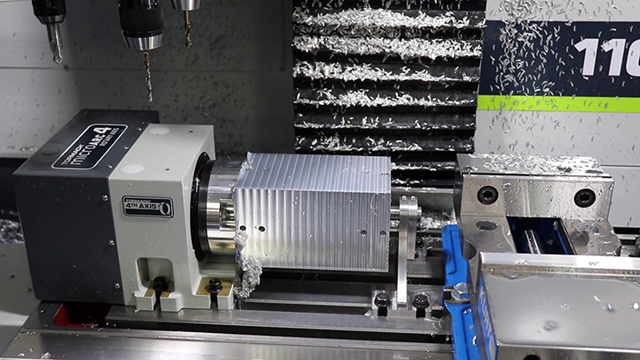
\includegraphics[width=0.7\linewidth]{imgs/4eje.png}
	\caption{Cuarto eje montado en fresa Tormach. \href{https://tormach.com}{Fuente}}
	\label{4ejefig}
\end{figure}

\section{Parámetros del proceso}

La cantidad de variables necesarias para definir una trayectoria de herramienta (\textit{toolpath}) en CNC es considerablemente mayor que en procesos como la impresión 3D. Esto se debe a que el mecanizado implica un contacto directo y forzado entre herramienta y material, lo que exige un control más fino sobre parámetros mecánicos, térmicos y dinámicos. Además, aspectos como la dirección del corte —por ejemplo, el corte en sentido convencional (\textbf{conventional milling}) versus el corte en sentido inverso o de trepado (\textbf{climb milling})— influyen directamente en la calidad del mecanizado, el esfuerzo sobre la herramienta y el acabado superficial.

En el \textit{corte convencional}, la herramienta avanza en dirección opuesta a la rotación del filo, lo cual es más estable para máquinas con juego mecánico, pero genera mayor fricción. En el \textit{corte en trepado}, el filo avanza en la misma dirección que gira, produciendo mejor acabado y menor desgaste, aunque requiere mayor rigidez de la máquina para evitar vibraciones.

Los dos parámetros cinemáticos fundamentales en el control de una operación CNC son las revoluciones del husillo y la {velocidad de avance lineal. Ambos están relacionados mediante el parámetro de avance por diente. Este parámetro condiciona directamente la carga sobre cada filo de corte, y a partir de él se derivan otras velocidades relevantes del proceso, como el avance en rampas o penetraciones verticales.

\begin{figure}[h!]
	\centering
	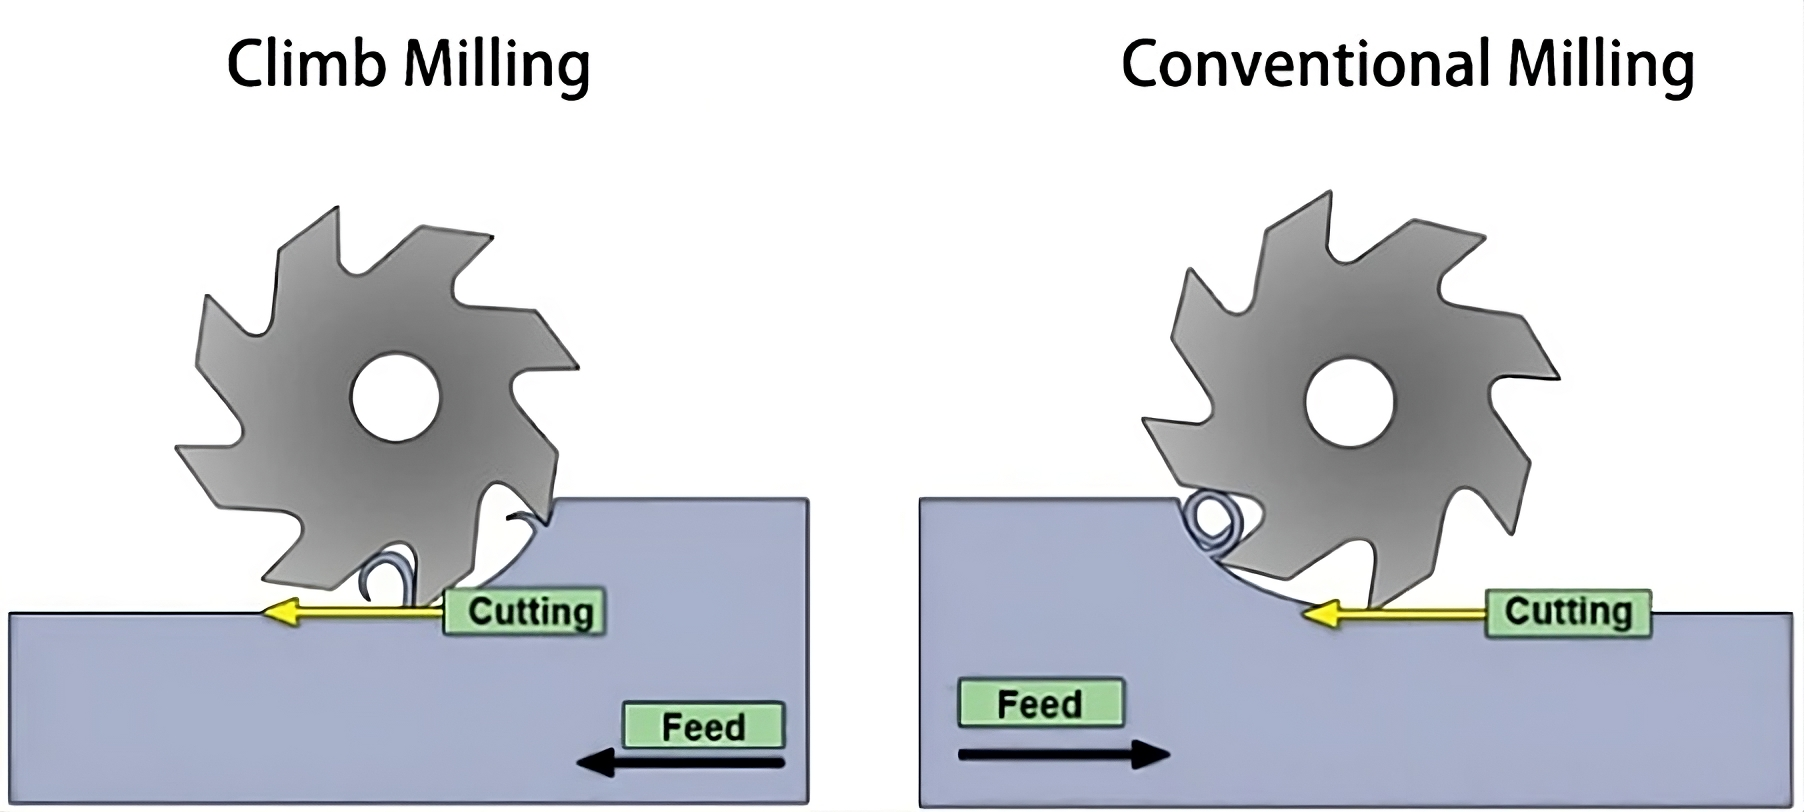
\includegraphics[width=0.8\linewidth]{imgs/climb.png}
	\caption{Dirección del corte, climbing y convencional. La dirección de avance es la del material. \href{https://kdmfab.com/climb-milling-vs-conventional-milling/}{Fuente}}
	\label{climbfig}
\end{figure}

En operaciones donde la herramienta penetra en el material de forma \textbf{vertical}, se utiliza la llamada \textbf{plunge speed}, que define la velocidad de avance exclusivamente en el eje Z. Este tipo de entrada puede ser agresivo y debe reservarse para herramientas con capacidad de corte axial.

Una alternativa más suave es la \textbf{entrada en rampa}, donde la herramienta desciende gradualmente mientras avanza. Esta estrategia proporciona mejores condiciones de corte inicial y se controla mediante la \textbf{ramp speed}, que es la velocidad de avance durante dicha trayectoria inclinada o helicoidal (Figura \ref{rampfig}).

\begin{figure}[h!]
	\centering
	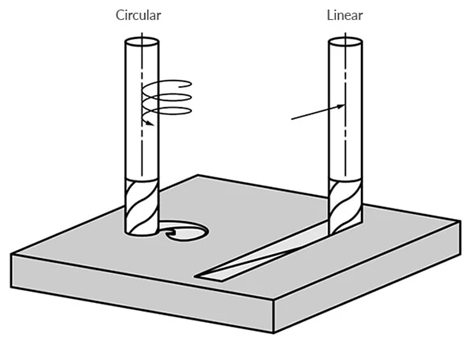
\includegraphics[width=0.55\linewidth]{imgs/ramp.png}
	\caption{Corte de entrada en rampa, helicoidal e inclinado. \href{https://www.harveyperformance.com/in-the-loupe/ramping-success/}{Fuente}}
	\label{rampfig}
\end{figure}

El MRR del proceso estará definido por la velocidad de corte, así como de la profundidad y del ancho, e impondrá las condiciones dinámicas en el sistema.

Estos parámetros también afectan la distribución térmica del proceso. Aunque la mayor parte del calor generado en el corte se transfiere a la viruta, una fracción significativa permanece en la herramienta y en la pieza. Incrementar la porción de la herramienta en contacto con el material puede ayudar a distribuir el calor sobre una mayor área, reduciendo los gradientes térmicos locales; sin embargo, las herramientas suelen ser de materiales con baja conductividad térmica, por lo que la disipación sigue siendo limitada.

Por ello, otro parámetro importante a considerar es el \textbf{control del refrigerante}, que aunque limitado desde el software CAM, puede activarse o desactivarse y configurarse en distintos modos de expulsión: refrigeración por inundación (\textit{flood}), nebulización (\textit{mist}), aire comprimido o refrigeración interna a través del husillo (\textit{through spindle coolant}, \textit{TSC}).

El \textit{toolpath} completo está compuesto por distintas fases de movimiento:
\begin{itemize}
	\item \textbf{Movimientos rápidos} (G0), utilizados para ubicar la herramienta en posición, fuera de contacto con la pieza;
	\item \textbf{Movimientos de aproximación o transición}, con velocidades reducidas para entrar en contacto con el material de forma controlada;
	\item \textbf{Movimientos de corte} (G1), donde se aplican los parámetros calculados para remover material.
\end{itemize}

Una consideración importante al momento de definir la estrategia de mecanizado en el entorno CAM es el uso de \textbf{tabs}, especialmente en el trabajo con planchas o placas delgadas. Un \textit{tab} es una pequeña porción del material que no se corta durante la operación, con el fin de mantener temporalmente un segmento de la pieza unido al stock. En la práctica, actúa como un punto de fijación pasivo.

\begin{figure}[h!]
	\centering
	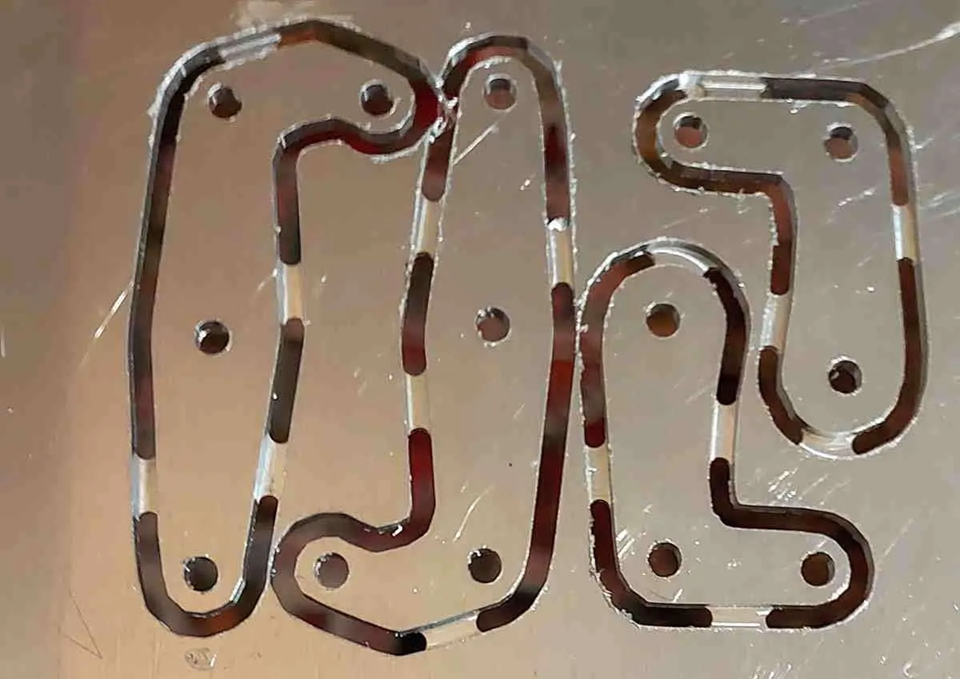
\includegraphics[width=0.55\linewidth]{imgs/tabs.png}
	\caption{Tabs en piezas fresadas sobre plancha de aluminio \href{https://www.glue-it.com/tools/milling-machines/cnc-holding-tabs/}{Fuente}}
	\label{tabsfig}
\end{figure}


El uso de tabs permite conservar la rigidez del sistema durante el mecanizado, evitando desplazamientos no deseados a medida que disminuye el área de contacto entre la pieza y el material base. Además, en muchos casos, elimina la necesidad de sistemas de fijación adicionales, simplificando el montaje.

Sin embargo, su utilización implica ciertas desventajas: aumenta el tiempo total de mecanizado y requiere operaciones de \textbf{postprocesado} manual, tales como la remoción del tab y la rectificación o acabado de la zona afectada para restaurar la geometría o el acabado superficial deseado.

Los parámetros mencionados tendrán un efecto directo en el tiempo de maquinado, no obstante, los tiempos de mecanizado CNC incluyen otras acciones de carácter preparativo o logístico, y se pueden separar como:

\begin{enumerate}
	\item \textbf{Tiempos de operación}: Corresponden al tiempo efectivo de corte durante cada trayecto programado en el CAM, según las estrategias seleccionadas y los parámetros de mecanizado.
	
	\item \textbf{Tiempos de preparación y montaje}: Incluyen el tiempo requerido para fijar/remover el stock a la mesa de trabajo, instalar sistemas de sujeción, alinear y referenciar la pieza, cambiar herramientas entre operaciones, realizar inspecciones intermedias y reorientar la pieza si es necesario.
	
	\item \textbf{Tiempos auxiliares e improductivos}: Agrupan todas aquellas pausas o actividades que, sin formar parte directa del mecanizado, afectan la duración total del proceso. Esto puede incluir tiempos de espera entre operaciones, limpieza de viruta, calibraciones, tiempos de calentamiento de la máquina, movimientos rápidos fuera de corte (reposicionamiento) y otros tiempos muertos asociados al entorno de trabajo.
\end{enumerate}

Finalmente, debe considerarse que cualquier incremento en los parámetros que aumentan la potencia requerida —como una mayor profundidad o ancho de corte— puede comprometer la calidad del mecanizado. A medida que se exige más al proceso, se incrementan fenómenos indeseables como la generación de calor, vibraciones, deflexión de la herramienta y desgaste prematuro. Estos efectos no solo afectan la precisión y el acabado superficial, sino que también ponen en tensión la capacidad del hardware disponible, por lo que es fundamental encontrar un equilibrio entre productividad, calidad y viabilidad técnica.


\section{Materiales y comportamiento frente al fresado}

\subsection{Maquinabilidad}

La maquinabilidad describe la facilidad con que un material puede ser mecanizado. No corresponde a una propiedad única, sino al resultado de múltiples características físicas, mecánicas y térmicas que influyen en la eficiencia del proceso. Puede abordarse tanto de forma cualitativa como cuantitativa, considerando factores como el desgaste de herramienta, la calidad superficial, la formación de viruta y el esfuerzo de corte requerido.

Para una comparación objetiva entre materiales, se emplean índices de maquinabilidad basados en parámetros medibles como la vida útil de la herramienta, la fuerza de corte o la tasa de remoción de material. En algunos casos, se utiliza un material de referencia (como el acero AISI 1112, al que se asigna un 100\% de maquinabilidad) para establecer relaciones relativas entre distintos materiales.

Entre los factores más relevantes que afectan la maquinabilidad se encuentran:

\begin{itemize}
	\item \textbf{Dureza:} Materiales más duros requieren mayores esfuerzos de corte y provocan mayor desgaste abrasivo en la herramienta.
	
	\item \textbf{Resistencia a la tracción:} Afecta directamente la fuerza necesaria para cortar el material; materiales con alta resistencia incrementan la carga sobre la herramienta.
	
	\item \textbf{Tenacidad:} Materiales tenaces tienden a formar virutas continuas difíciles de controlar, y presentan mayor tendencia a la adhesión sobre el filo.
	
	\item \textbf{Conductividad térmica:} Una baja conductividad concentra el calor en la zona de corte, reduciendo la vida útil de la herramienta y afectando la estabilidad térmica del proceso.
	
	\item \textbf{Coeficiente de fricción:} Influye en el comportamiento tribológico entre la herramienta y la pieza. Altos valores generan mayor calor y aceleran el desgaste.
	
	\item \textbf{Formación de viruta:} La facilidad con que el material se fragmenta en virutas cortas mejora la evacuación y reduce los problemas de acumulación y recalentamiento.
	
	\item \textbf{Composición química:} Elementos de aleación o impurezas pueden formar fases duras o abrasivas que afectan negativamente la maquinabilidad.
	
	\item \textbf{Microestructura:} Granos finos suelen facilitar el corte, mientras que estructuras heterogéneas o con fases duras dificultan el proceso.
	
	\item \textbf{Deformabilidad plástica:} Materiales muy dúctiles pueden sufrir deformación en lugar de corte limpio, lo que deteriora el acabado superficial.
	
	\item \textbf{Contenido de inclusiones:} Algunas inclusiones (como sulfuros) pueden actuar como lubricantes internos, facilitando el corte.
	
	\item \textbf{Tendencia a la adhesión:} Materiales como el titanio o el aluminio puro pueden soldarse al filo, alterando la geometría efectiva de corte.
\end{itemize}

Estas propiedades influyen de forma directa sobre la selección de herramientas, parámetros de corte, refrigeración y estrategias de mecanizado, y se manifiestan de manera concreta según el tipo de material empleado. A continuación, se examinan algunos materiales representativos y sus implicancias prácticas durante el fresado.

\subsection{Materiales comunes y su respuesta al fresado}

\begin{itemize}
	\item \textbf{Dureza y resistencia a la deformación plástica:} Materiales con alta resistencia mecánica, como el acero inoxidable AISI 304 o el titanio grado 5, generan mayores fuerzas de corte y temperaturas en la zona de corte. Esto acelera el desgaste por abrasión y adhesión, y puede inducir vibraciones o flexión en herramientas de pequeño diámetro.
	
	\item \textbf{Tenacidad y ductilidad:} En materiales dúctiles como el nylon 6 o el polietileno de alta densidad (HDPE), se produce una viruta continua con tendencia a la adhesión sobre el filo de corte. Esta acumulación puede modificar la geometría efectiva de corte y deteriorar la calidad superficial.
	
	\item \textbf{Abrasividad:} Compuestos con cargas minerales, como ciertos plásticos reforzados con fibra de vidrio (GF30) o matrices poliméricas con sílice, provocan desgaste abrasivo severo, especialmente en herramientas sin recubrimiento. Esto es crítico en operaciones prolongadas o de producción continua.
	
	\item \textbf{Conductividad térmica:} Materiales con baja conductividad térmica, como el acero inoxidable o los composites termoestables, concentran el calor en la zona de corte. Esto favorece el ablandamiento localizado, pero también puede generar tensiones térmicas, deformaciones y deterioro del filo de herramienta por difusión o oxidación.
	
	\item \textbf{Coeficiente de dilatación térmica:} En materiales como el aluminio 6061, con alto coeficiente de expansión térmica, pueden observarse cambios dimensionales durante el mecanizado prolongado, especialmente en piezas de gran volumen o cuando no se emplea refrigeración efectiva.
\end{itemize}

La acumulación de viruta sobre el filo de corte, también conocida como formación de borde de aportación (\textit{built-up edge}), representa una condición crítica en el fresado, especialmente en materiales dúctiles como aleaciones de aluminio o termoplásticos. Esta acumulación modifica la geometría efectiva de la herramienta, alterando el ángulo de ataque y reduciendo la capacidad de corte. Como consecuencia, se generan fuerzas de corte inestables, incremento en la generación de calor y deterioro de la calidad superficial de la pieza. Además, el desprendimiento intermitente del material adherido puede producir defectos en la superficie mecanizada y acelerar el desgaste por impacto en el filo activo. 

\begin{figure}[h!]
	\centering
	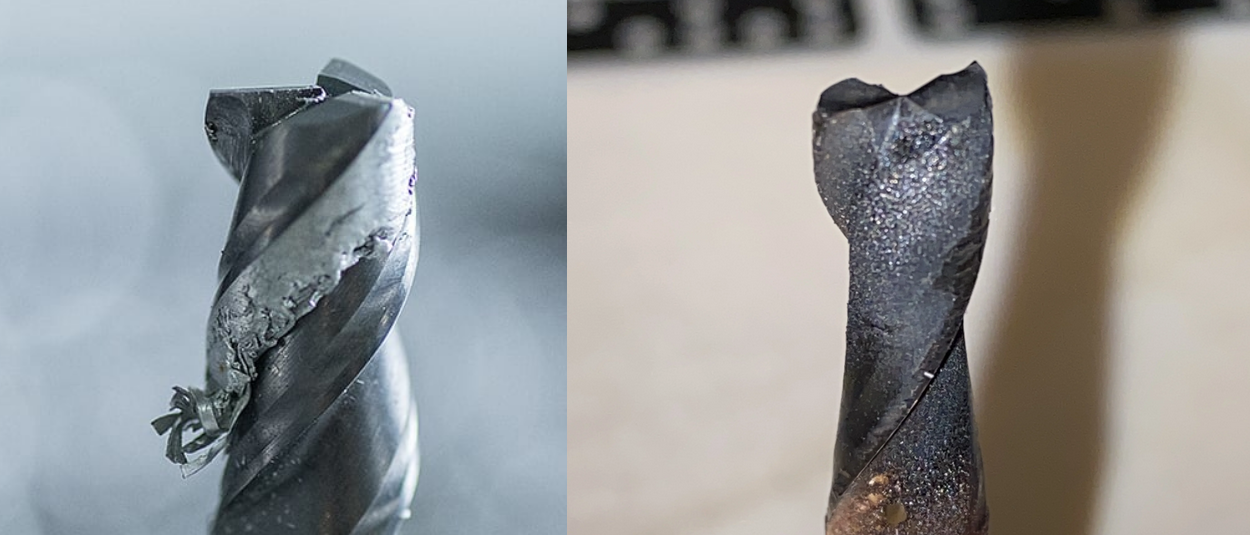
\includegraphics[width=0.8\linewidth]{imgs/edge.png}
	\caption{Fresa plana con acumulación de material en el filo, y fresa quemada. \href{https://www.routerforums.com}{Fuente}}
	\label{edgefig}
\end{figure}

La acumulación de viruta puede minimizarse mediante el uso de herramientas con recubrimientos de baja adhesión, control de la temperatura mediante refrigeración, y ajustes en los parámetros de corte para evitar el régimen de corte discontinuo que favorece este fenómeno.

\subsection{Recomendaciones según material}

Las propiedades anteriores se traducen en decisiones concretas sobre herramientas, geometrías, recubrimientos y parámetros de corte. A continuación, se presentan algunos valores representativos:

\begin{itemize}
	\item \textbf{Acero al carbono (AISI 1045):} Se mecaniza con fresas de carburo con recubrimiento TiAlN o similar. Velocidades de corte típicas entre 90 y 140 m/min, con avances por diente de 0{,}05--0{,15} mm. Requiere refrigeración continua para controlar el calor y prolongar la vida de la herramienta.
	
	\item \textbf{Acero inoxidable (AISI 304):} Material austenítico con baja conductividad térmica y tendencia a la deformación por endurecimiento. Se recomiendan herramientas de carburo recubiertas con geometrías de corte positivas. Velocidades de corte más bajas (60--100 m/min) y avances moderados. La refrigeración es obligatoria para evitar acumulación térmica.
	
	\item \textbf{Aluminio 6061:} Permite altas velocidades de corte (300--600 m/min) debido a su baja dureza y alta conductividad térmica. Se recomiendan fresas de 2 o 3 filos, sin recubrimiento o con recubrimientos que reduzcan la adhesión (ZrN, DLC). El uso de refrigerante depende de la velocidad y de la evacuación de viruta.
	
	\item \textbf{Nylon (PA6):} Material blando, de baja rigidez y alta tenacidad. Requiere filos agudos, avances reducidos y velocidades intermedias (80--150 m/min). El mecanizado en seco puede generar acumulación de viruta por electrificación o fusión localizada; se recomienda aire comprimido o refrigeración con MQL.
	
	\item \textbf{Composites reforzados (GF30, CFRP):} Presentan abrasividad alta. Se emplean herramientas PCD o fresas de carburo con recubrimientos duros. Velocidades de corte bajas, avances moderados y mínima profundidad de corte para evitar delaminación o desintegración del material.
\end{itemize}

\section{Flujo del proceso}

\subsection{Consideraciones previas}

La planificación de una operación CNC puede abordarse de diversas maneras, dependiendo de las capacidades de las máquinas, las herramientas disponibles y las propiedades del material a mecanizar. Estas restricciones, en muchos casos, pueden condicionar decisiones de diseño geométrico o incluso la selección del material base.

Incluso en ausencia de limitaciones técnicas, el diseño debe ser evaluado en función de las condiciones mínimas que impone el mecanizado. Entre ellas se encuentran evitar bordes internos perfectamente rectos —que no pueden generarse con herramientas rotativas—, garantizar accesibilidad en todas las zonas a cortar, y considerar la disponibilidad comercial del formato de material seleccionado.

El formato del stock debe presentar una dimensión característica (espesor, diámetro) ligeramente superior a la requerida por la pieza final, permitiendo el mecanizado de las superficies funcionales sin comprometer sus dimensiones ni aumentar innecesariamente el tiempo de corte. Alternativamente, puede optarse por adaptar el diseño a espesores comerciales estándar. En este sentido, es importante considerar que, a medida que aumenta el espesor del material, su costo se incrementa considerablemente y su disponibilidad en el mercado local puede verse limitada. Particularmente, planchas de más de 20~mm en ciertos materiales pueden no estar fácilmente disponibles, dependiendo del contexto geográfico y de los proveedores existentes.

La accesibilidad a las zonas de corte es uno de los factores más determinantes para la efectividad y eficiencia del fresado. Las tecnologías sustractivas, especialmente aquellas con arquitectura cartesiana, presentan limitaciones claras para ejecutar trayectorias de corte en planos oblicuos o perpendiculares a la superficie de trabajo.

Por ejemplo, en una fresadora CNC cartesiana, una operación en el plano superior de la pieza puede realizarse sin dificultad. Sin embargo, un patrón de perforaciones laterales, aunque geométricamente simple, requerirá rotar el material para dar acceso a esa cara. Esto implica tiempos adicionales de reconfiguración, necesidad de fijaciones auxiliares (\textit{fixtures}) y riesgo de pérdida de precisión en la referencia de origen. Por esta razón, estas fresadoras son habitualmente denominadas \textbf{máquinas 2.5D}, aludiendo a su capacidad limitada de acceso volumétrico.

Esta limitación no se presenta en fresadoras de 4 o 5 ejes, donde el cabezal o la pieza pueden rotarse para acceder a múltiples caras sin cambiar la referencia de origen. No obstante, estas máquinas implican un mayor costo, complejidad operativa y requerimientos de programación más avanzados, lo que restringe su uso principalmente a entornos industriales o especializados.


\subsection{CAM}

La mayoría de los softwares CAD actuales integran un CAM para corte CNC, luego, será sencillo pasar de la revisión del diseño al entorno de manufactura (y viceversa). Los pasos en el CAM tendrán el siguiente orden general:

\begin{enumerate}
	\item Definir el tamaño del stock y su posición relativa con la pieza.
	\item Definir el origen y las direcciones del sistema de coordenadas relativo.
	\item Definir operaciones, herramientas y parámetros de corte.
	\item Chequear simulaciones.
	\item Postprocesar el código G respecto a la máquina a utilizar.
\end{enumerate}

En general, el stock puede representarse como el formato comercial real que se montará en la máquina, o bien como un volumen virtual mínimo que contenga completamente la geometría de la pieza. No obstante, utilizar el formato completo del material disponible es lo más recomendable, ya que obliga a considerar desde el inicio aspectos prácticos del proceso, como la estrategia de fijación y la interacción del stock con el sistema de sujeción. Además, incorporar este volumen en el modelo facilita la simulación y la verificación del mecanizado.

El \textbf{origen relativo} (también llamado \textit{punto cero de pieza} o \textit{workpiece zero}) es la referencia a partir de la cual se calcularán todas las trayectorias de herramienta en el entorno CAM. Este debe ser un punto físicamente alcanzable por la herramienta o por los accesorios de sondaje utilizados para la referencia en la máquina CNC. Comúnmente, se selecciona un vértice del stock debido a su facilidad de acceso y consistencia geométrica. 

Es fundamental que el sistema de coordenadas definido en el software CAM coincida con la orientación real del sistema de la máquina CNC a utilizar. Una mala correspondencia entre ambos sistemas puede derivar en errores de simulación, colisiones o cortes fuera de la pieza. 

Una vez definido el sistema de coordenadas, se procede a establecer las distintas \textbf{operaciones de mecanizado}, seleccionando para cada una:
\begin{itemize}
	\item La estrategia de corte 
	\item Los parámetros de corte apropiados (avances, profundidades, velocidades).
	\item La herramienta correspondiente, intentando reducir al mínimo el número total de herramientas diferentes, lo cual optimiza los tiempos de cambio. 
\end{itemize}

A cada herramienta se le asigna un identificador único (ID), el cual será reconocido por el control de la máquina y permitirá realizar cambios automáticos o manuales de manera organizada. Idealmente, se agrupan en secuencia todas las operaciones que involucren a la misma herramienta.

Al finalizar la definición de cada operación, se ejecuta una \textbf{simulación parcial} del trayecto de herramienta, lo que permite:
\begin{itemize}
	\item Verificar visualmente la trayectoria generada.
	\item Detectar colisiones potenciales con el stock, fijaciones o la propia herramienta.
	\item Confirmar el volumen de material removido, que será tenido en cuenta para las operaciones posteriores.
\end{itemize}

Estas simulaciones pueden mejorarse al incorporar modelos del portaherramientas, del husillo e incluso del sistema de sujeción, lo cual permite realizar simulaciones más fieles al entorno real de trabajo. También es posible integrar parámetros específicos de la máquina seleccionada, lo que ayuda a predecir comportamientos dinámicos como límites de velocidad, aceleraciones y movimientos de seguridad.

El proceso se repite iterativamente hasta que la simulación global sea coherente con los objetivos de calidad superficial, precisión y tiempo de mecanizado estimado.

Finalmente, se genera el \textbf{código G}, ya sea como un archivo único o como una serie de bloques independientes según las operaciones programadas. Es fundamental asegurarse de utilizar el \textbf{postprocesador correcto}, que adapta el código generado al dialecto específico del controlador CNC correspondiente (como Fanuc, Haas, Siemens, etc.), garantizando así la compatibilidad y el correcto funcionamiento en la máquina de destino.

\subsection{Preparación del corte}

Antes de ejecutar cualquier trayecto de herramienta en la máquina CNC, es necesario llevar a cabo una serie de actividades fundamentales que permiten garantizar la precisión, seguridad y repetibilidad del proceso. Esta etapa se conoce como la \textbf{preparación del corte} o \textbf{set-up del proceso}, y puede involucrar tanto tareas físicas en la máquina como procedimientos de medición y calibración.

El primer paso es montar correctamente la materia prima (\textbf{stock}) sobre la mesa de trabajo de la máquina. Para ello se emplea un \textbf{sistema de fijación} adecuado a la geometría y características del material: mordazas, placas de vacío, bridas, sistemas modulares, tornillos de sujeción o fijaciones personalizadas. Es crucial que la fijación:
\begin{itemize}
	\item Sea suficientemente rígida para evitar desplazamientos durante el mecanizado.
	\item No interfiera con las trayectorias de la herramienta.
	\item Permita el acceso a las caras que deben ser trabajadas.
\end{itemize}

En caso de requerirse múltiples operaciones o cambios de orientación de la pieza, deben planificarse también los métodos de realineación y fijación secundaria.

Cada herramienta de corte debe montarse sobre su correspondiente portaherramientas (collet, pinza ER, mandril hidráulico, etc.), y luego en el husillo o en el almacén automático de la máquina (ATC). Es fundamental identificar correctamente cada herramienta con un número de herramienta (T) correspondiente al ID asignado en el programa CAM.

A continuación, se deben \textbf{calibrar los offsets de herramienta}, es decir, registrar la longitud efectiva de cada herramienta con respecto a un punto de referencia fijo. Esta operación se puede realizar:

\begin{itemize}
	\item Manualmente, tocando con la herramienta una superficie de referencia y registrando la distancia.
	\item Usando un \textbf{dispositivo de medición automática} (tool setter), que mide la longitud y opcionalmente el diámetro de forma automatizada.
\end{itemize}

Para que el programa de mecanizado se ejecute correctamente, es necesario alinear el sistema de coordenadas del programa con el de la máquina. Esto se logra a través de un procedimiento de \textbf{sondaje} o \textbf{referenciación}, donde se determina el \textbf{cero pieza} o \textit{workpiece zero}.

Este punto de origen debe coincidir con el definido en el CAM y puede ubicarse en:
\begin{itemize}
	\item Una esquina del stock (común en fresado).
	\item El centro de una cara (común en torneado).
	\item Una superficie intermedia determinada por una sonda táctil o medidor de altura.
\end{itemize}

El cero pieza se define normalmente utilizando una sonda, un reloj comparador o métodos manuales de aproximación con herramientas de referencia (papel, bloques patrón, etc.).

Una vez completado el montaje y la referenciación, se recomienda realizar una \textbf{simulación en seco} o \textit{dry run}, es decir, una ejecución del programa sin contacto con la pieza (con la herramienta elevada), para verificar:

\begin{itemize}
	\item Que no existan colisiones.
	\item Que los desplazamientos y cambios de herramienta sean correctos.
	\item Que el origen y los offsets estén correctamente definidos.
\end{itemize}

Esta etapa es crítica para prevenir errores que puedan dañar la pieza, la herramienta o la máquina.


\subsection{Ejecución}

Una vez que la máquina ha sido preparada, se procede a cargar el programa de mecanizado (código G) mediante la interfaz del controlador. Antes de iniciar, se verifica que los identificadores de las herramientas utilizados en el CAM correspondan con los efectivamente montados en la máquina, tanto en términos de posición como de offset. Confirmada esta correspondencia, se puede ejecutar la primera operación.

El nivel de automatización de la máquina determina el grado de intervención del operador. En sistemas manuales o semiautomáticos, el operador puede estar encargado de:

\begin{itemize}
	\item Realizar el cambio de herramientas entre operaciones.
	\item Marcar o redefinir el origen de coordenadas tras cada reconfiguración.
	\item Reorientar la pieza de trabajo según sea necesario para acceder a otras caras.
\end{itemize}

En sistemas con cambiadores automáticos de herramientas (ATC) y sondas de palpado, estas tareas pueden realizarse sin intervención directa. Sin embargo, se debe seguir asegurando la correcta correspondencia entre el programa y los elementos montados.

Durante la ejecución, la interfaz HMI permite el monitoreo de variables relevantes como:

\begin{itemize}
	\item Avance del programa (línea actual del código G).
	\item Estados del husillo, ejes y refrigeración.
	\item Alarmas o advertencias del sistema.
\end{itemize}

En ciertos controladores es posible modificar parámetros en tiempo real, como la velocidad de avance o la velocidad del husillo. Estas modificaciones pueden utilizarse para ajustar el comportamiento del proceso frente a condiciones no previstas o cambios en el material.

En caso de detectar inconsistencias durante la ejecución, ya sea visuales, sonoras o mediante advertencias del sistema, el operador puede pausar o detener el proceso mediante los controles disponibles, según el protocolo de operación de la máquina.


\subsection{Postprocesado}

Las operaciones de \textbf{postprocesado} en una pieza mecanizada tienen como objetivo ajustar sus características finales, especialmente cuando el mecanizado principal no alcanza por sí solo los requisitos dimensionales, funcionales o estéticos especificados.

Entre las tareas más comunes de postprocesado se incluyen:

\begin{itemize}
	\item \textbf{Rectificación}: proceso de remoción fina de material mediante abrasivos, utilizado para alcanzar tolerancias dimensionales estrictas, corregir deformaciones menores o mejorar la geometría final de la pieza.
	
	\item \textbf{Acabado superficial}: se aplican técnicas como lijado, pulido o chorro abrasivo para alcanzar el nivel de rugosidad requerido, ya sea por motivos funcionales (fricción, contacto, adherencia) o estéticos.
	
	\item \textbf{Suavizado de bordes}: mediante operaciones como biselado o redondeo (manual o automatizado), se eliminan aristas vivas que podrían generar problemas de ensamblaje, acumulación de tensiones o riesgo de corte.
	
	\item \textbf{Remoción de rebabas y \textit{tabs}}: especialmente comunes en procesos de corte 2D o en piezas fijadas mediante \textit{tabs}, estas protuberancias deben eliminarse mediante corte secundario, limado o fresado puntual, seguido de una corrección local del acabado superficial.
	
	\item \textbf{Limpieza}: se retiran residuos como viruta, refrigerante, polvo metálico o aceites de corte, mediante métodos mecánicos, térmicos o químicos, dependiendo del material de la pieza y los requerimientos del proceso posterior (como pintura, ensamblaje o control dimensional).
\end{itemize}

Un aspecto fundamental del postprocesado es el \textbf{control metrológico}, el cual permite verificar que la pieza final cumpla con las tolerancias y especificaciones dimensionales establecidas en el diseño. Para ello, se emplean instrumentos como calibres, micrómetros, relojes comparadores, proyectores de perfiles o sistemas de medición por coordenadas (CMM, \textit{Coordinate Measuring Machines}).

\subsection{Medición de calidad}

Una vez finalizado el mecanizado, se miden los siguientes parámetros para verificar la conformidad de la pieza con las especificaciones técnicas:

\begin{itemize}
	\item \textbf{Tolerancias dimensionales:} Se determina la conformidad de dimensiones críticas (longitudes, diámetros, espesores, radios) con los valores establecidos en el diseño. La medición se realiza utilizando micrómetros, pie de metro y máquinas de medición por coordenadas (CMM).\\
	\textit{Ajuste:} En caso de desviaciones dimensionales, se puede ajustar la velocidad de giro (RPM), reducir la velocidad de avance, disminuir la profundidad de corte o utilizar herramientas de menor diámetro para mejorar la precisión. También se revisa la fijación de la pieza y la calibración de la máquina para minimizar vibraciones y movimientos no deseados.
	
	\item \textbf{Rugosidad superficial:} Se cuantifica la textura superficial mediante parámetros como Ra, utilizando rugosímetros o profilómetros. Este parámetro describe las irregularidades y variaciones de la superficie en escala micrométrica.\\
	\textit{Ajuste:} Para reducir la rugosidad, se puede disminuir el avance por diente, aumentar las RPM, seleccionar herramientas con geometría de corte más adecuada (por ejemplo, fresas de mayor filo o con recubrimiento especial) o implementar pases de acabado con menor profundidad y \textit{stepover}. También es posible añadir procesos secundarios como pulido o rectificado.
	
	\item \textbf{Defectos superficiales:} Se inspeccionan visualmente o con métodos ópticos defectos tales como quemaduras, marcas de herramientas, rebabas y grietas. Estos se asocian a condiciones del proceso de corte y del estado de la herramienta.\\
	\textit{Ajuste:} Se recomienda aumentar el flujo y tipo de refrigerante, reducir la velocidad de corte y avance para disminuir la generación de calor, cambiar o afilar la herramienta para evitar desgastes y vibraciones, y mejorar la sujeción de la pieza para evitar movimientos durante el mecanizado.
	
	\item \textbf{Propiedades mecánicas y microestructurales:} En ciertos casos, se evalúan características como dureza y estructura interna a través de ensayos destructivos o no destructivos, para verificar la integridad del material tras el mecanizado.\\
	\textit{Ajuste:} Si se detectan alteraciones, se pueden aplicar tratamientos térmicos posteriores (recozido, temple, revenido), controlar la temperatura y la velocidad de corte para evitar sobrecalentamiento, y seleccionar estrategias de mecanizado que reduzcan tensiones residuales, como cortes más suaves y menos profundos.
	
\end{itemize}

\section{Operaciones comunes}

\subsection{Etapas de mecanizado}

El proceso de mecanizado generalmente se divide en tres etapas principales que permiten optimizar la eficiencia, la precisión y la calidad superficial de la pieza fabricada: \textbf{desbaste} (\textit{roughing}), \textbf{semifinishing} y \textbf{acabado} (\textit{finishing}).

En el desbaste se realiza la remoción de grandes volúmenes de material con el objetivo de aproximar la forma final de la pieza. Las condiciones de corte son agresivas, con profundidades y avances altos, buscando maximizar la tasa de arranque de material. Debido a la alta carga sobre la herramienta y las mayores vibraciones presentes, la precisión dimensional y el acabado superficial no son prioritarios en esta fase. Se emplean herramientas robustas y estrategias que priorizan la rapidez y la eficiencia en la eliminación del material sobrante.

El semifinishing busca refinar la geometría aproximada obtenida durante el desbaste, eliminando las irregularidades y preparando la pieza para la etapa final. Los parámetros de corte se ajustan para reducir la carga sobre la herramienta y mejorar la precisión dimensional. Se disminuyen las profundidades y avances para disminuir la generación de vibraciones y mejorar la estabilidad del proceso. El acabado superficial comienza a mejorar, aunque generalmente no se alcanzan los niveles de calidad requeridos para el producto final.

Finalmente, en el acabado se realizan cortes con profundidades muy pequeñas y velocidades de avance reducidas para obtener la máxima precisión dimensional y un acabado superficial óptimo. Se emplean herramientas especializadas, generalmente afiladas y geometrías que favorecen un corte limpio y sin marcas. El objetivo principal es cumplir con las tolerancias más estrictas y obtener superficies lisas que cumplan con los requerimientos funcionales y estéticos de la pieza.

Estas etapas definen de manera fundamental el equilibrio entre productividad y calidad en el proceso de mecanizado, determinadas directamente por parámetros como el \textit{stock to leave}, la profundidad de corte y el \textit{stepover}.

El parámetro \textit{stock to leave} representa la cantidad de material residual que se deja intencionalmente sobre la geometría final. Este valor asegura un margen para las siguientes etapas de mecanizado, facilitando un acabado más preciso. Habitualmente, se procura mantener este valor bajo, con el fin de minimizar la carga de trabajo en las herramientas de acabado, que suelen ser más delicadas y costosas.

Por su parte, la profundidad de corte afecta directamente el tiempo total de operación, ya que determinará el número de niveles o pasadas necesarias para completar el mecanizado. Además, su influencia sobre la resolución geométrica dependerá en gran medida de la estrategia de corte empleada, pudiendo impactar en la calidad dimensional de la pieza.

Finalmente, el \textit{stepover} o solape lateral incide directamente en la calidad superficial de la pieza mecanizada, al influir en la rugosidad generada. Este efecto es particularmente evidente en fresas de bola, donde un \textit{stepover} inadecuado puede dar lugar a patrones de crestas y valles, tal como se ilustra en la Figura \ref{bols}.
 
\subsection{Operaciones 2D}

En el fresado CNC bidimensional (2D), la herramienta se desplaza principalmente en los ejes \textit{X} e \textit{Y}, con profundidades constantes en el eje \textit{Z}. Estas operaciones son las más sencillas y frecuentes en corte CNC, especialmente al momento de trabajar con planchas de material. Las más comunes son:

\begin{itemize}
	
	\item \textbf{Contorneado (Contour):} Esta operación consiste en un movimiento de la herramienta tangencial a un contorno por el exterior o interior de una geometría, permitiendo cortar la pieza a lo largo de su perímetro. Puede realizarse a distintas profundidades por pasos sucesivos.
	
	\item \textbf{Refrentado (Facing):} También conocido como \comillas{careado}, esta operación elimina material de la parte superior de una pieza para obtener una superficie plana. Se utiliza generalmente como operación inicial para nivelar la superficie del material antes de otras operaciones más precisas.
	
	\item \textbf{Cajoneras (Pocketing):} Esta operación desbasta material dentro de una región cerrada, sin cortar completamente el perímetro exterior de la pieza. Se emplea para crear cavidades, alojamientos o áreas huecas.
	
	\item \textbf{Taladrado (Drilling):} Consiste en crear un orificio cilíndrico en el material mediante una broca. Puede realizarse en una sola pasada o en pasos sucesivos si el orificio es profundo.
	
	 \item \textbf{Roscado (Tapping):} Consiste en crear una rosca interna (hilo) en un orificio para permitir la inserción de tornillos o pernos. Puede realizarse mediante machos de roscar (taps) o herramientas de roscado helicoidal, coordinando la rotación del cabezal y el paso en Z.
	
\end{itemize}

\subsection{Operaciones 3D}

En el fresado tridimensional, la trayectoria de la herramienta se adapta a la geometría de superficies complejas, permitiendo el mecanizado de formas libres u orgánicas. Los sistemas CAM ofrecen diversas estrategias de generación de trayectorias, que definen el patrón de desplazamiento de la herramienta sobre la pieza. La elección adecuada de la estrategia impacta directamente en la eficiencia del mecanizado, la calidad del corte y la duración de la herramienta.

A continuación se describen las estrategias más comunes:

\begin{itemize}
	\item \textbf{Movimiento paralelo a un plano (Parallel / Raster):} La herramienta se desplaza en líneas paralelas dentro de un plano definido (usualmente XY), ajustando su posición en el eje Z según la geometría de la superficie. Es eficiente para superficies de curvatura suave y amplia.
	
	\item \textbf{Movimiento por niveles de altura (Z-Level / Contour):} Se generan trayectorias horizontales a diferentes alturas Z, siguiendo las secciones horizontales de la superficie. Es especialmente útil para paredes inclinadas o escalonadas.
	
	\item \textbf{Movimiento en espiral (Spiral):} La herramienta sigue una trayectoria helicoidal continua, desde el centro hacia los bordes (o viceversa), adaptándose a la forma tridimensional. Esta estrategia reduce los cambios de dirección y puede mejorar la estabilidad del corte.
	
	\item \textbf{Movimiento radial (Radial):} Las trayectorias se extienden desde un punto central hacia el exterior como radios. Es adecuada para superficies con simetría circular o geometrías centradas.
	
	\item \textbf{Festoneado (Scallop):} Se genera una trayectoria que mantiene constante la distancia entre pasadas a lo largo de la superficie, siguiendo su forma natural. Produce un patrón de corte más uniforme en superficies curvas, y se adapta bien a transiciones complejas.
	
	\item \textbf{Rampa (Ramp):} La herramienta penetra progresivamente en el material siguiendo una trayectoria inclinada, en lugar de descender verticalmente. Esta estrategia se utiliza tanto para ingresar al material como para realizar cortes continuos, minimizando esfuerzos axiales y reduciendo el riesgo de daño en herramientas frágiles.
\end{itemize}



